\documentclass[a4paper,oneside]{article}

\usepackage[utf8]{inputenc}
\usepackage[T2A]{fontenc}
\usepackage[english,russian]{babel}

\usepackage{amsmath}
\usepackage{mathtools}
\usepackage{amsfonts}
\usepackage{enumitem}
\usepackage{amsthm}
\usepackage{minted}
\setminted{fontsize=\small, breaklines=true, style=emacs, linenos}
\usepackage{graphicx}
\graphicspath{ {./images/} }
\usepackage{float}

\newtheorem{theorem}{Теорема}[subsection]
\newtheorem*{theorem*}{Теорема}

% --- Определение --- %
\theoremstyle{definition}
\newtheorem{definition}{Определение}[subsection]
\newtheorem*{definition*}{Определение}
% ------------------- %

\title{{Теория кодирования и сжатия информации}\\{Лабораторная работа №2}}
\author{Гущин Андрей, 431 группа, 1 подгруппа}
\date{\the\year{} г.}

\begin{document}

\maketitle

\section{Задача}

Разработать программу осуществляющую архивацию и разархивацию текстового файла
используя алгоритм Фано. Программы архивации и разархивации должны быть
представлены отдельно и работать независимо друг от друга. Определить для
данного шифра характеристики 1 (коэффициент сжатия) и 2 (скорость сжатия). К
работе необходимо прикрепить отчет и программный проект.


\section{Алгоритм}

Алгоритм Фано заключается в создании нового кода для каждого встречающегося
в тексте символа на основе частоты встречи этого символа.

Алгоритм состоит из следующих шагов:
\begin{enumerate}
  \item Вычислить частоты всех встретившихся символов;
  \item Отсортировать полученный список по невозрастанию;
  \item
    Подразбивать список на две части так, чтобы суммы вероятностей в
    этих частях были примерно равны;
  \item
    На основе попадания в левую или правую часть подразбивки элементы
    переносятся в левую или правую ветвь дерева;
  \item На основе дерева вычислить код для каждого символа.
\end{enumerate}


\section{Тестирование}

Для проверки программы были использованы тестовые тексты 1 (рис.
\ref{fig:test_1}) и 6 (рис. \ref{fig:test_6}). Можно заметить,
что после распаковки архива полученный файл совпадает с исходным (проверка
с помощью утилиты diff). Также можно заметить, что для файлов малого размера
архив увеличивает их размер за счёт метаданных.

\begin{figure}[H]
  \centering
  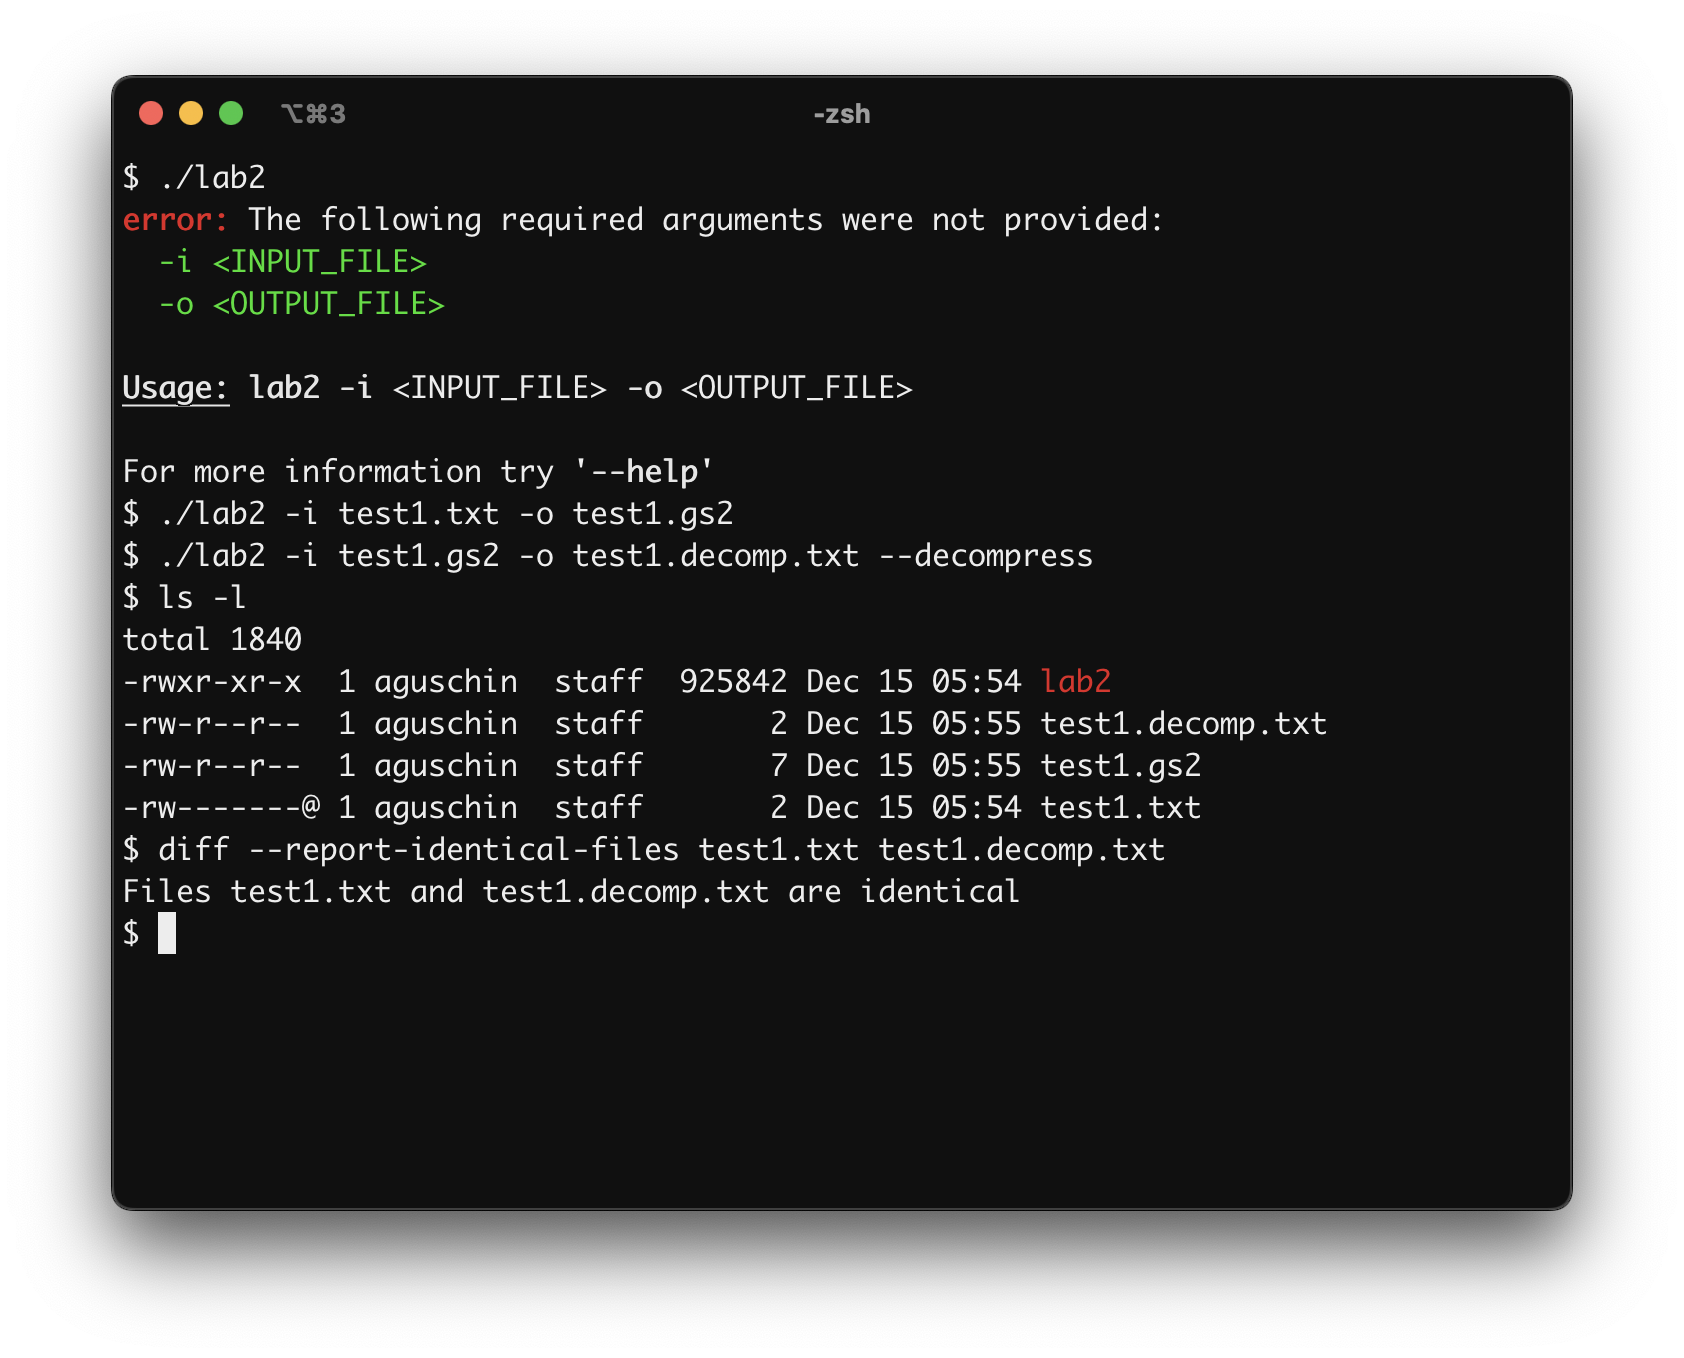
\includegraphics[width=0.9\textwidth]{test1.png}
  \caption{Сжатие текста Тест\_1.txt}
  \label{fig:test_1}
\end{figure}

\begin{figure}[H]
  \centering
  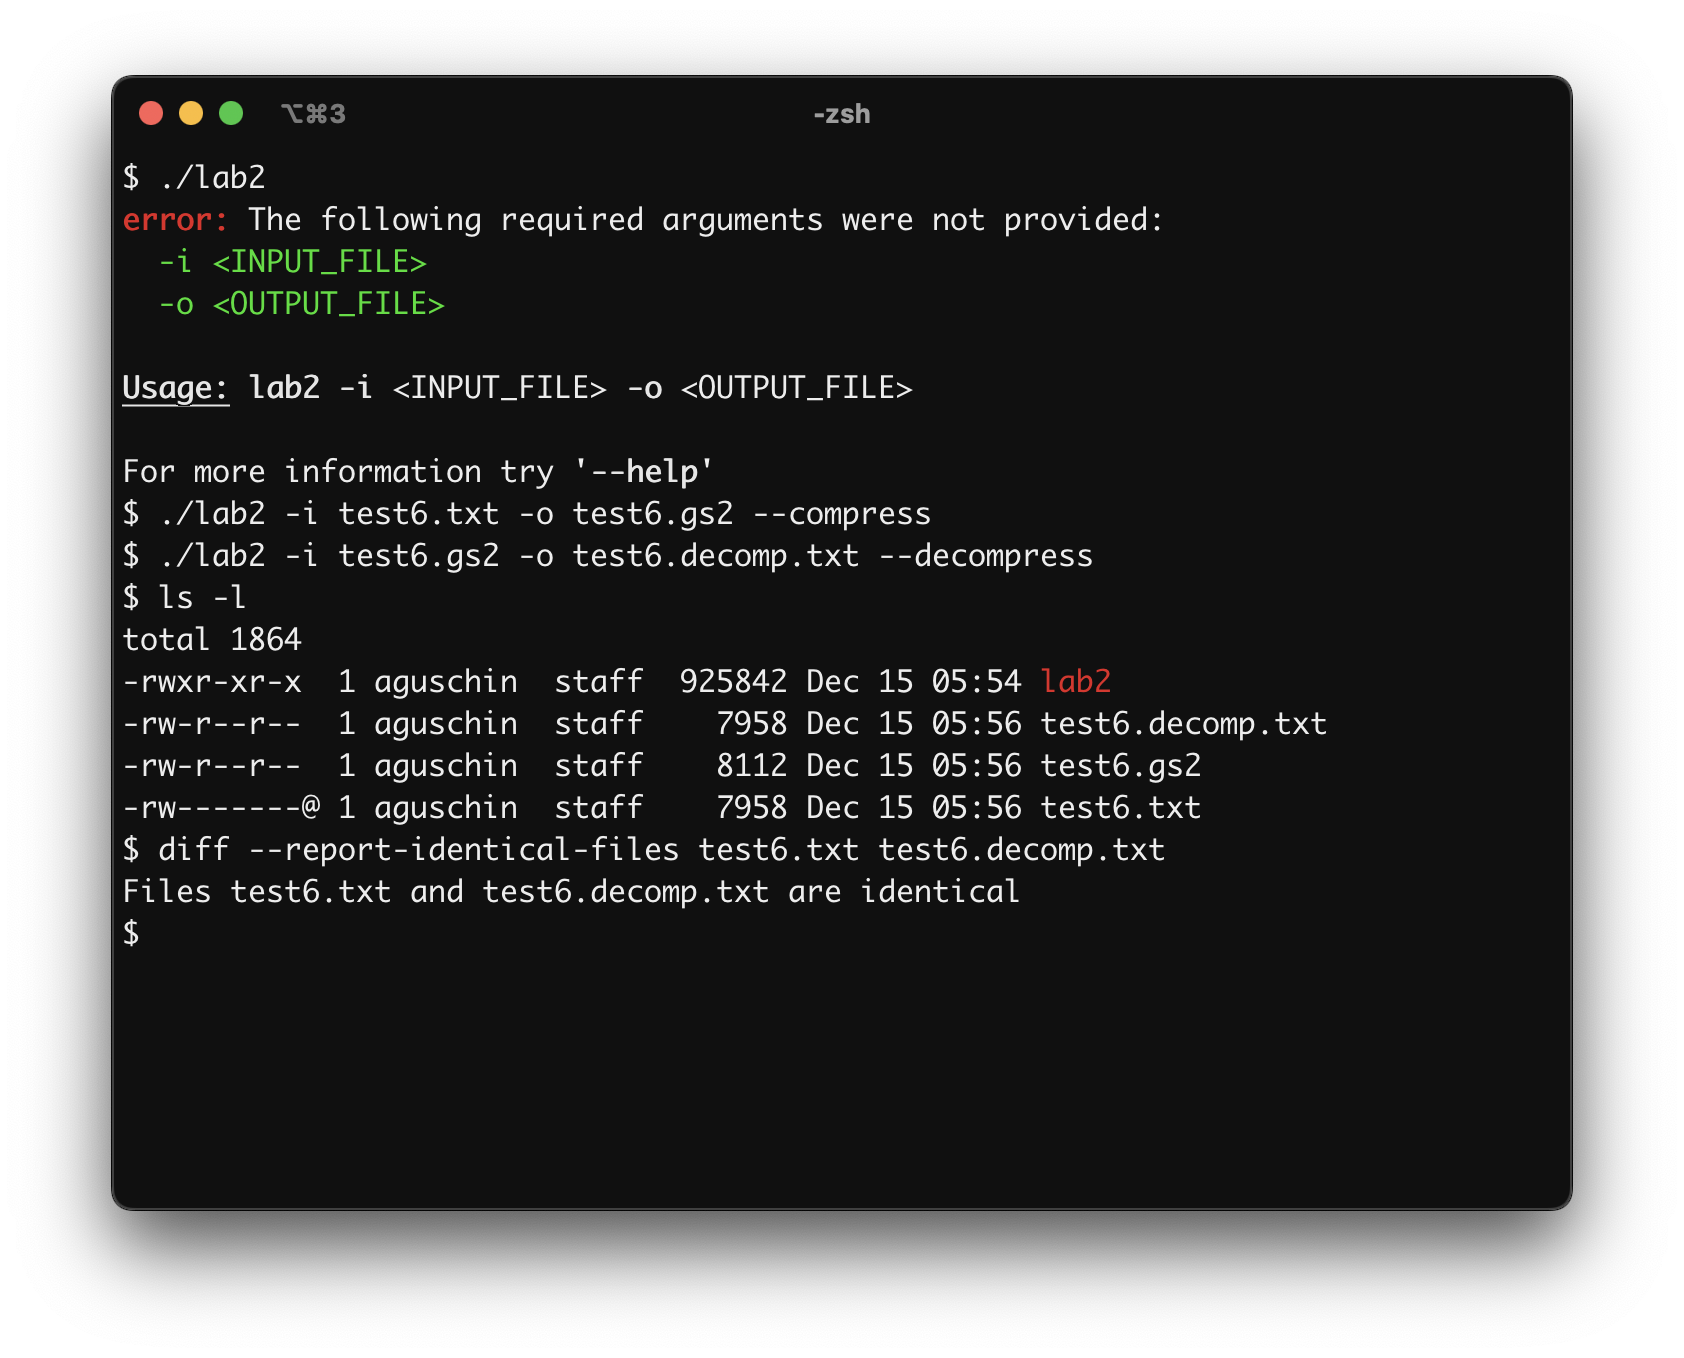
\includegraphics[width=0.9\textwidth]{test6.png}
  \caption{Сжатие текста Тест\_6.txt}
  \label{fig:test_6}
\end{figure}


\section{Вычисленные характеристики}

\subsection{Характеристика 1 (Коэффициент сжатия)}

Результаты применения программы к каждому из тестовых текстовых файлов занесены
в таблицу \ref{tbl:results}.

\begin{table}[H]
  \small
  \centering
  \begin{tabular}{|c|c|c|c|}
    \hline
    Название     & Исходный размер, байт & Сжатый размер, байт & Коэффициент \\ \hline \hline
    Тест\_1.txt  & 2           & 7           & 0.28571   \\ \hline
    Тест\_2.txt  & 33          & 92          & 0.3587    \\ \hline
    Тест\_3.txt  & 2739        & 2029        & 1.34993   \\ \hline
    Тест\_4.txt  & 330         & 48          & 6.875     \\ \hline
    Тест\_5.txt  & 59          & 169         & 0.34911   \\ \hline
    Тест\_6.txt  & 7958        & 8112        & 0.98102   \\ \hline
    Тест\_7.txt  & 138245      & 122970      & 1.12422   \\ \hline
    Тест\_8.txt  & 574426      & 511681      & 1.12263   \\ \hline
    Тест\_9.txt  & 2752        & 349         & 7.88539   \\ \hline
    Тест\_10.txt & 2814        & 368         & 7.64674   \\ \hline
  \end{tabular}
  \caption{результаты тестирования}
  \label{tbl:results}
\end{table}

\subsection{Характеристика 2 (Скорость сжатия)}

Для тестирования скорости сжатия использовался произвольный двоичный
файл размера 76450438 байт ($\approx$73 мегабайта). В результате пяти
последовательных запусков, среднее время запаковки файла составило 4.31
секунды, среднее время распаковки составило 5 секунд.

Таким образом, средняя скорость сжатия составила 16.9162 Мбайт в секунду, а
средняя скорость разжатия составила 14.58176 Мбайт в секунду.


\section{Реализация}

Программа реализована на языке программирования Rust с использованием библиотеки
clap для чтения параметров командной строки. Сборка производится с помощью
программы cargo, поставляющейся вместе с языком.

\subsection{Содержимое файла weighted.rs}
\inputminted{rust}{../../lab2/src/weighted.rs}

\subsection{Содержимое файла fano.rs}
\inputminted{rust}{../../lab2/src/fano.rs}

\subsection{Содержимое файла main.rs}
\inputminted{rust}{../../lab2/src/main.rs}

\subsection{Содержимое файла Cargo.toml}
\inputminted{toml}{../../lab2/Cargo.toml}

\end{document}
